\documentclass[12pt,a4paper]{report}
\usepackage[brazil]{babel}
\usepackage[]{algorithm}
\usepackage[]{algorithmic}
\usepackage[style=numeric,backend=biber]{biblatex}
\usepackage[utf8]{inputenc}
\usepackage{kpfonts}
\usepackage[T1]{fontenc}
\usepackage{wrapfig}
\usepackage{graphicx}
\usepackage{enumerate}
\usepackage{subcaption}
\usepackage{float}
\usepackage{caption}
\usepackage{listings}
\usepackage{lipsum}
\usepackage{amsthm}
\usepackage{amssymb}
\usepackage{bm}
\usepackage{color}
\usepackage{afterpage}
\usepackage[inline]{enumitem}
\usepackage{pdflscape}
\usepackage{listingsutf8}
\usepackage{siunitx}
\usepackage{bashful}

\graphicspath{ {./images/} }

\lstset{frame=tb,
  aboveskip=2mm,
  belowskip=2mm,
  showstringspaces=false,
  columns=flexible,
  basicstyle=\footnotesize,,
  numbers=left,
  numbersep=5pt,
  stepnumber=1,
  breaklines=true,
  keepspaces=true,
  breakatwhitespace=true,
  showtabs=false,  
  tabsize=2
}

% Definindo estilo para os códigos
\definecolor{mGreen}{rgb}{0,0.6,0}
\definecolor{mGray}{rgb}{0.5,0.5,0.5}
\definecolor{mPurple}{rgb}{0.58,0,0.82}
\definecolor{dkgreen}{rgb}{0,0.6,0}
\definecolor{backgroundColour}{rgb}{0.97,0.97,0.97}

\lstset{basicstyle=\ttfamily,
    backgroundcolor=\color{backgroundColour},   
    commentstyle=\color{mGreen},
    keywordstyle=\color{magenta},
    numberstyle=\tiny\color{mGray},
    commentstyle=\color{dkgreen},
    stringstyle=\color{mPurple},
    basicstyle=\footnotesize,
    breakatwhitespace=false\textbf{,}         
    breaklines=true,                 
    captionpos=b,                    
    keepspaces=true,                 
    numbers=left,                    
    numbersep=5pt,                  
    showspaces=false,                
    showstringspaces=false,
    showtabs=false,                  
    tabsize=2,
    language=bash
}

\lstdefinestyle{BStyle}{
    backgroundcolor=\color{backgroundColour},  
    showstringspaces=false,
    numbers=none,
    language=bash
}

\pagenumbering{arabic}
\renewcommand{\thesection}{\arabic{section}}

\bibliography{ref}
\renewcommand{\contentsname}{Sumário}{\thispagestyle{empty}}
\renewcommand{\baselinestretch}{1.5} 

\begin{document}

\begin{titlepage}
    \begin{center}
        \vspace*{1cm}
        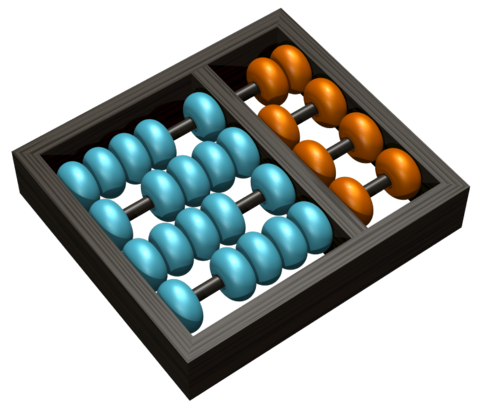
\includegraphics[width=0.25\textwidth]{Logo}\\
        \vspace{1.5cm}
        \Huge
    	\textbf{MC833 Relatório 2 \\
        Ferramentas e Sniffers} \\
        \vspace{1.5cm}
        \Large
        \textbf{Aluno}: Fábio Camargo Ricci\\
        \textbf{RA}: 170781\\
        \vspace{1.2cm}
    	\Large 
    	Instituto de Computação\\
    	Universidade Estadual de Campinas\\
    	\vspace{1.5cm}
        Campinas, 2 de Setembro de 2021.
    \end{center}
\end{titlepage}
\tableofcontents
\clearpage

\newcommand{\shellcmd}[1]{\texttt{\footnotesize\# #1}}%estilizando citação de comandos do shell

\section{Questões}

\begin{enumerate}
    \item Considere para esta questão o comando ifconfig.
    \begin{enumerate}
        \item Qual opção deve ser usada para exibir informações sobre todas as interfaces de rede?
        \item O que deve ser feito para exibir somente informações de uma interface específica? 
    \end{enumerate}
    
    \item Através da execução do comando nslookup seguido dos parâmetros adequados, responda à seguinte questões:
    \begin{enumerate}
        \item Quais são os endereços IP do host www.unicamp.br?
        \item Há alguma vantagem em haver mais de um endereço IP?
    \end{enumerate}
    
    \item Através da execução do comando traceroute seguido dos parâmetros adequados, responda à seguinte questão:
    \begin{enumerate}
        \item Quantos roteadores estão entre a sua estação e o host www.amazon.com? Pelos nomes dos roteadores, quantos deles estão localizados no Brasil?
    \end{enumerate}
    
    \item Através da execução do comando telnet, seguido dos parâmetros adequados, responda às seguintes questões:
    \begin{enumerate}
        \item É possível conectar-se com este comando em um servidor HTTP? Se sim, como deve se executar o comando para conectar-se no host www.amazon.com na porta padrão do HTTP?
        \item Caso não haja um servidor escutando na porta passada pelo comando telnet, o que ocorre? Justifique.
        \item A qual a camada da rede o telnet pertence?
    \end{enumerate}
    
    \item Acesse o site da DAC (https://www.dac.unicamp.br/) e, em paralelo em um terminal, verifique a saída do comando netstat. Quais são as informações fornecidas a respeito da conexão ao site da DAC?
    
    \item Considere a ferramenta TCPDUMP, e responda às seguintes questões:
    \begin{enumerate}
        \item Utilizando o TCPDUMP corretamente com os filtros é possível somente capturar o tráfego HTTPS? Se sim, execute o comando junto com os filtros e anexe uma figura que comprove sua resposta no relatório. Se sua resposta foi não, então justifique-a.
        \item Utilizando o comando TCPDUMP seguido dos parâmetros corretos imprima somente os pacotes superiores a 64 bits. Indique qual foi a sequência de comandos utilizada. 
        \item Utilizando o TCPDUMP seguido de filtros, imprima somente os resultados que tiverem a flag ‘ACK’. Insira o comando seguido dos filtros e uma figura no seu relatório para comprovar o sucesso.
    \end{enumerate}
    
    \item Considere a ferramenta Wireshark para responder às questões a seguir:
    \begin{enumerate}
        \item Comparado às demais ferramentas apresentadas na aula de MC833 descreva quais são principais diferenças e vantagens de usar o Wireshark? Escolha pelo menos uma ferramenta/sniffer e elabore uma tabela comparativa para responder a questão. 
        \item Com o conhecimento adquirido sobre ferramentas e sniffers responda:
        \begin{enumerate}
            \item Em uma rede com vários processos acontecendo ao mesmo tempo é possível gerenciar de forma isolada um único processo específico na rede utilizando ferramentas/sniffers apresentados nesta disciplina? Se sim, quais ferramentas  e/ou sniffers você usaria? Justifique sua resposta. (OBS: Não é necessário apresentar comandos ou prints)
        \end{enumerate}
    \end{enumerate}
\end{enumerate}

\section{Respostas}

\begin{enumerate}
    \item
    \begin{enumerate}
        \item Deve ser utilizada a opção -a (ex: ifconfig -a), mostrando todas as interfaces de rede, sendo utilizadas ou não
        \item Deve ser utilizado o nome da interface (ex: ifconfig eth0), mostrando apenas as informações da interface eth0
    \end{enumerate}
    
    \item
    \begin{enumerate}
        \item O endereço IP do host www.unicamp.br é 143.106.143.187. Foi executado o comando nslookup www.unicamp.br
        \\
        \\
        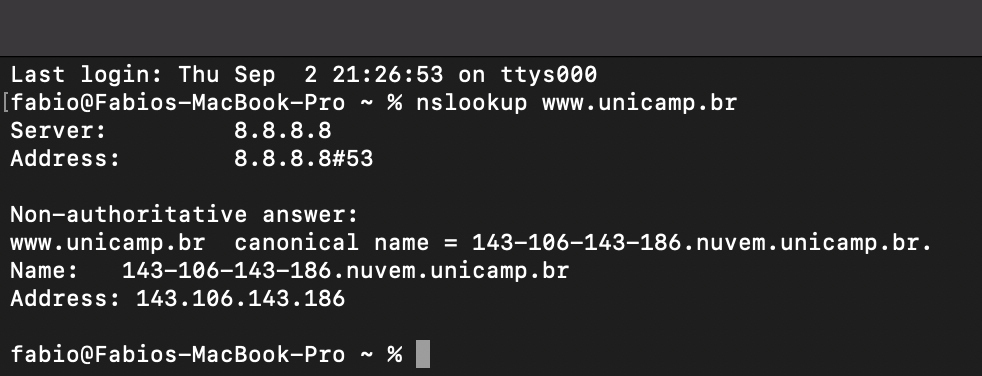
\includegraphics[width=10cm, height=4cm]{2a.png}
        \item Sim, com mais de um endereço IP, a escalabilidade de um serviço ou servidor se torna mais fácil, possivelmente aumentando o alcance geográfico e a distribuição de carga do mesmo.
    \end{enumerate}
    
    \item
    \begin{enumerate}
        \item A flag -I indica para o comando traceroute utilizar o protocolo ICMP, a fim de tentar passar por possíveis firewalls (muitos deles deixam conexões ICMP passarem) que barrem a conexão TCP que o traceroute faça com os roteadores.
        \\
        \\
        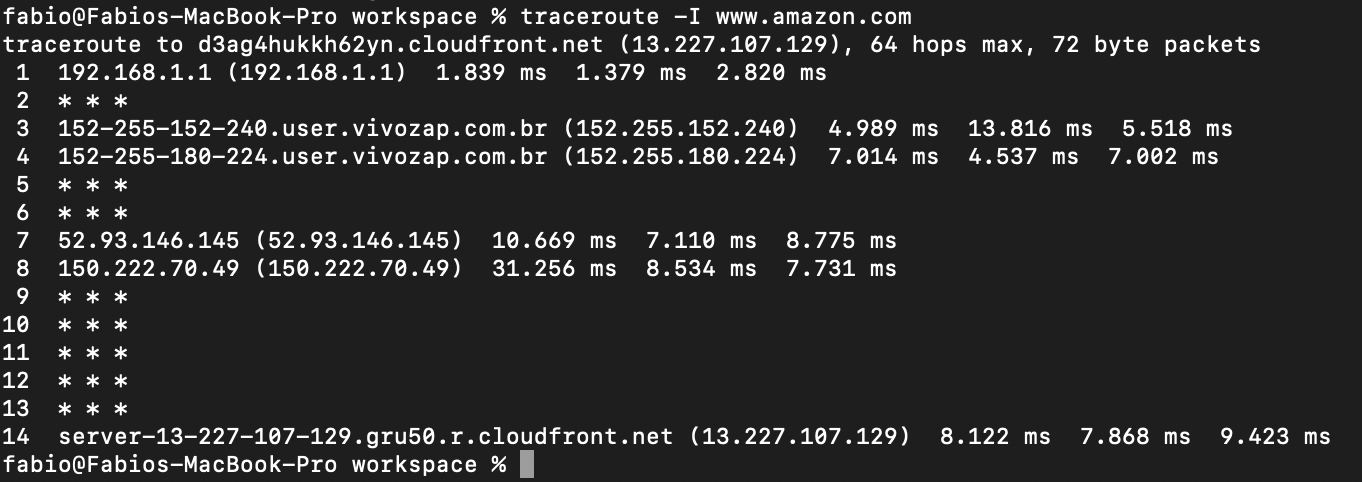
\includegraphics[width=12cm, height=5cm]{3a.png}
        \\
    	Existem 5 roteadores entre a minha estação e o host www.amazon.com. Pelo nome dos roteadores apresentados, 3 deles estão localizados no Brasil, o primeiro (residencial) e os 2 seguintes da Vivo.
    \end{enumerate}
    
    \item
    \begin{enumerate}
        \item Sim, é possível, basta executar: 
        \\
        telnet www.amazon.com 80
        \\
        \\
        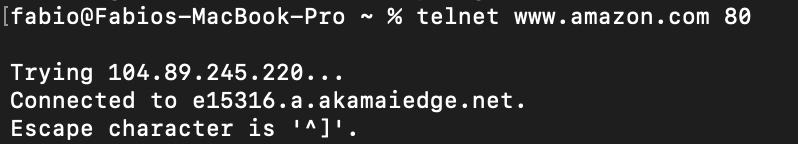
\includegraphics[width=10cm, height=2cm]{4a.png}
        \item Caso não haja um servidor escutando na porta passada, o comando telnet falhará e encerrará a conexão. Foi passada a porta 5434 arbitrariamente esperando-se que não havia servidor escutando nessa porta    
        \\
        \\
        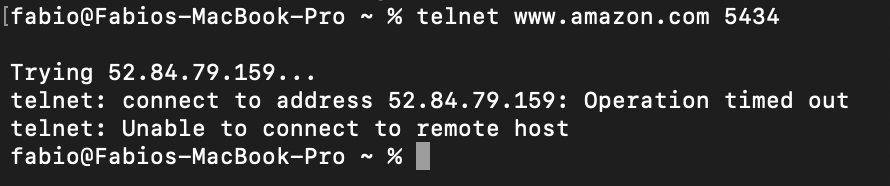
\includegraphics[width=10cm, height=2cm]{4b.png}
        \item O telnet é um protocolo que pertence à camada de aplicação
    \end{enumerate}
    
    \item Executando-se o comando nslookup www.dac.unicamp.br, descobrimos o endereço IP do site da DAC (143.106.227.165). Com essa informação, podemos executar o comando.
    \\
    netstat -an | grep 143.106.227.165
    \\
    -a para apenas conexões ativas.
    \\
    -n para evitar que o netstat tente determinar o nome dos hosts para endereços IPs externos, diminuindo consideravelmente o tempo de execução.
    \\        
    \\
    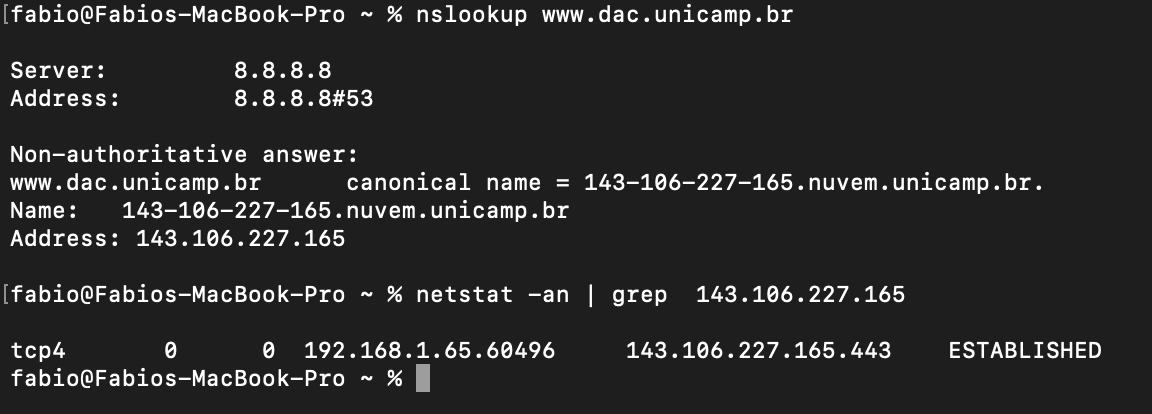
\includegraphics[width=10cm, height=4cm]{5.png}
    \\
    Conseguimos informações como, os protocolos (Proto) sendo utilizados (tcp4 - TCP IPv6), quantos dados estão na fila para serem recebidos (Recv-Q) e (Send-Q) enviados (0 e 0), o endereços e portas locais e externos da conexão com o servidor (192.168.1.65:60496 e 143.106.227.165:443 respectivamente) e o status da conexão (ESTABLISHED). 
    
    \item 
    \begin{enumerate}
        \item Sim é possível, uma vez que nunca haverá tráfego HTTPS em outra porta (protocolo). Assim, basta executar:
        \\
        sudo tcpdump -i any 'tcp port 443' -w ./http-only.pcap
        \\
        -i: qualquer interface de rede
        \\
        'tcp port 443': todas as conexões TCP na porta 443 (padrão HTTPS)
        \\
        \\
        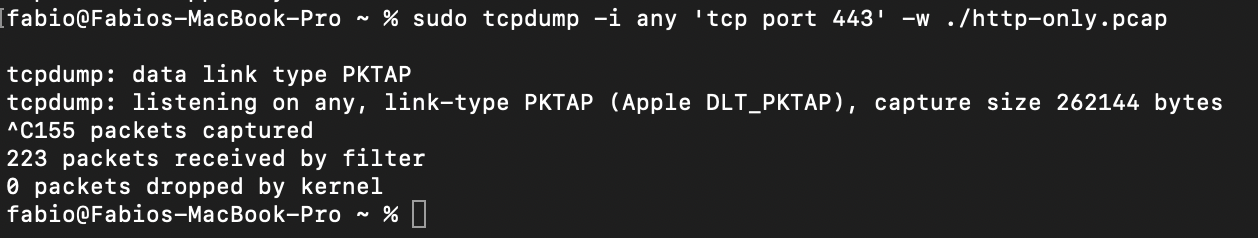
\includegraphics[width=12cm, height=3cm]{6a.png}
        \item sudo tcpdump -i any 'len > 64' -w ./greater64.pcap
        \\
        -i: qualquer interface de rede
        \\
        'len > 64': todos os pacotes com tamanho maior que 64 bytes
        \\
        \\
        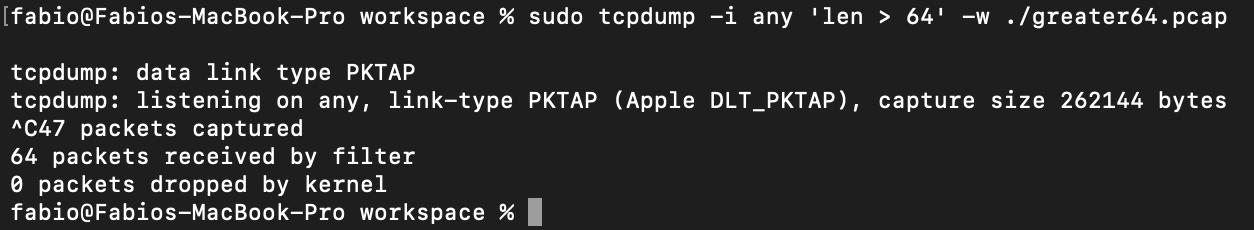
\includegraphics[width=12cm, height=3cm]{6b.png}
        \item sudo tcpdump -i any 'tcp[tcpflags] == tcp-ack' -w ./ack.pcap
        \\
        -i: qualquer interface de rede
        \\
        'tcp[tcpflags] == tcp-ack': Filtra todos os pacotes TCP que possuem a flag ACK
        \\
        \\
        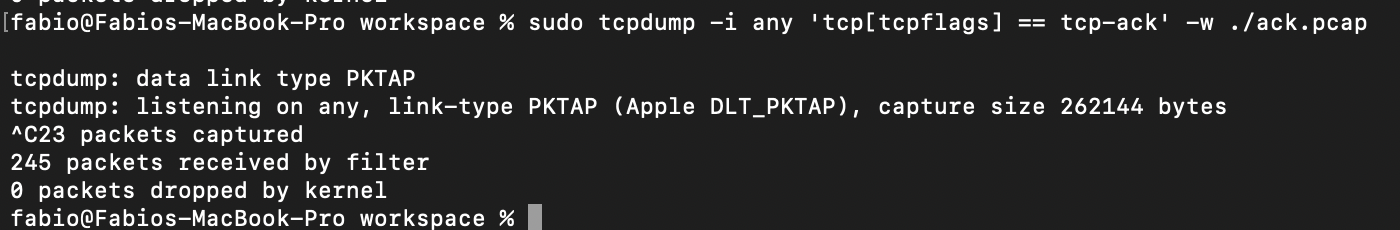
\includegraphics[width=12cm, height=3cm]{6c.png}
    \end{enumerate}
    
    \item
    \begin{enumerate}
        \item 
        \begin{tabular}{ | m{2cm} | m{5cm}| m{4cm} | } 
            \hline
             & \textbf{Wireshark} & \textbf{tcpdump} \\
            \hline
            \textbf{Interface} & Interface gráfica (GUI) & CLI (linha de comando) \\
            \hline
            \textbf{Análise de pacotes} & Possibilidade de análise de payload de pacotes, mesmo sendo criptografados (chaves são necessárias) ou se protocolos de transporte de arquivo (STMP, HTTP, etc) & Apenas análise simples como tipos de tráfego (ex: DNS queries) \\
            \hline
            \textbf{Interfaces de redes} & Possui interfaces de redes avançadas &Apenas possui interfaces de redes convencionais \\ 
            \hline
            \textbf{Filtros} & Fornece filtros complexos & Fornece apenas filtros simples \\
            \hline
        \end{tabular}
        \\
        \\
        A principal vantagem de se utilizar o Wireshark é a interface gráfica e possibilidade de filtros avançados/análise de pacotes que ele fornece, sendo possível ter uma visão mais detalhada de todas as informações disponíveis na rede.
        \item
        \begin{enumerate}
            \item Sim. Utilizando o tcpdump ou wireshark, por exemplo, é possível verificar todos os processos na rede, o process ID de cada um, e as portas sendo utilizadas pelos mesmos, também havendo a possibilidade da aplicação de filtros e análise de pacotes (no caso do wireshark).
        \end{enumerate}
    \end{enumerate}
\end{enumerate}

\end{document}
